% :( No more epic citations in final report
%\epigraph{You're the chosen one, Cuckoo.}{Adriaan}

For the Proof of Concept (PoC), Cuckoo \cite{cuckoo} will be used. Cuckoo is a malware analysis system that runs malware in a virtual environment, tracks its behaviour and reports these results to the user.\\

Cuckoo was choosen because it already implements a great deal of the prerequisites of the algorithm, discussed in \ref{sec:prereq}. Cuckoo, through Cuckoomon \cite{cuckoomon}, provides a series of hooks which monitors calls between the browser and the operating system.

These hooks, conveniently, also monitor the network calls made by the browser. Although only Internet Explorer is supported by Cuckoo, due to the scope of the project, this is not a problem.

\subsubsection{Prerequisites and changes}

As explained in \ref{sec:brie}, Internet Explorer uses Windows' ``Schannel'' \cite{schannel} to encrypt HTTP requests and decrypt HTTP responses. This will allow us to monitor traffic on the operating system level without any need for a proxy to decrypt the traffic.

As already explained, Cuckoo uses Cuckoomon, which uses hooks to monitor calls, to keep track of the browser activity. Besides adding a few new hooks and deleting irrelevant hooks for drive-by downloads, nothing major has to be changed to Cuckoomon. The list of hooks to be added and to be deleted can be found in Appendix \ref{cuckoomonmods}.

The current development version, \texttt{1.2-dev},  only accepts one URL at a time. To allow for concurrently visiting multiple websites in one sandbox environment, Cuckoo has to be extended.

\subsubsection{The setup}
\label{sec:setup}

To test the algorithm, we will use the adapted Cuckoo with Virtualbox as the sandbox environment. As the virtual machine's operating system, we will use Windows 7 as this is widely used and also frequently targetted by malware developers. As the browser, we will use Internet Explorer 8\todo{Ook misschien verwijzen naar de theorie dat doordat IE zijn process model deze het makkelijkst te monitoren is?} to actually allow the malware to successfully perform the drive-by download.

The adapted Cuckoo will be provisioned with the top 20 of visited websites in the Netherlands\footnote{http://www.alexa.com/topsites/countries/NL}, and one website who serves a drive-by download which spawns processes.

The structure of the graph will be tree-like, as suggested in \ref{sec:algos2}. Figure \ref{fig:alg_tree} shows an example graph of a website with a drive-by download.

After confirming that the PoC works, a comparison will be made with two malware analysis systems: Cuckoo and Anubis.

\setcounter{savepage}{\arabic{page}}
\stepcounter{savepage}
\pagebreak

\pagenumbering{gobble}
\newgeometry{left=3cm,top=0.1cm,bottom=0.1cm}
\begin{figure}[h]
    \centering
    \centerline{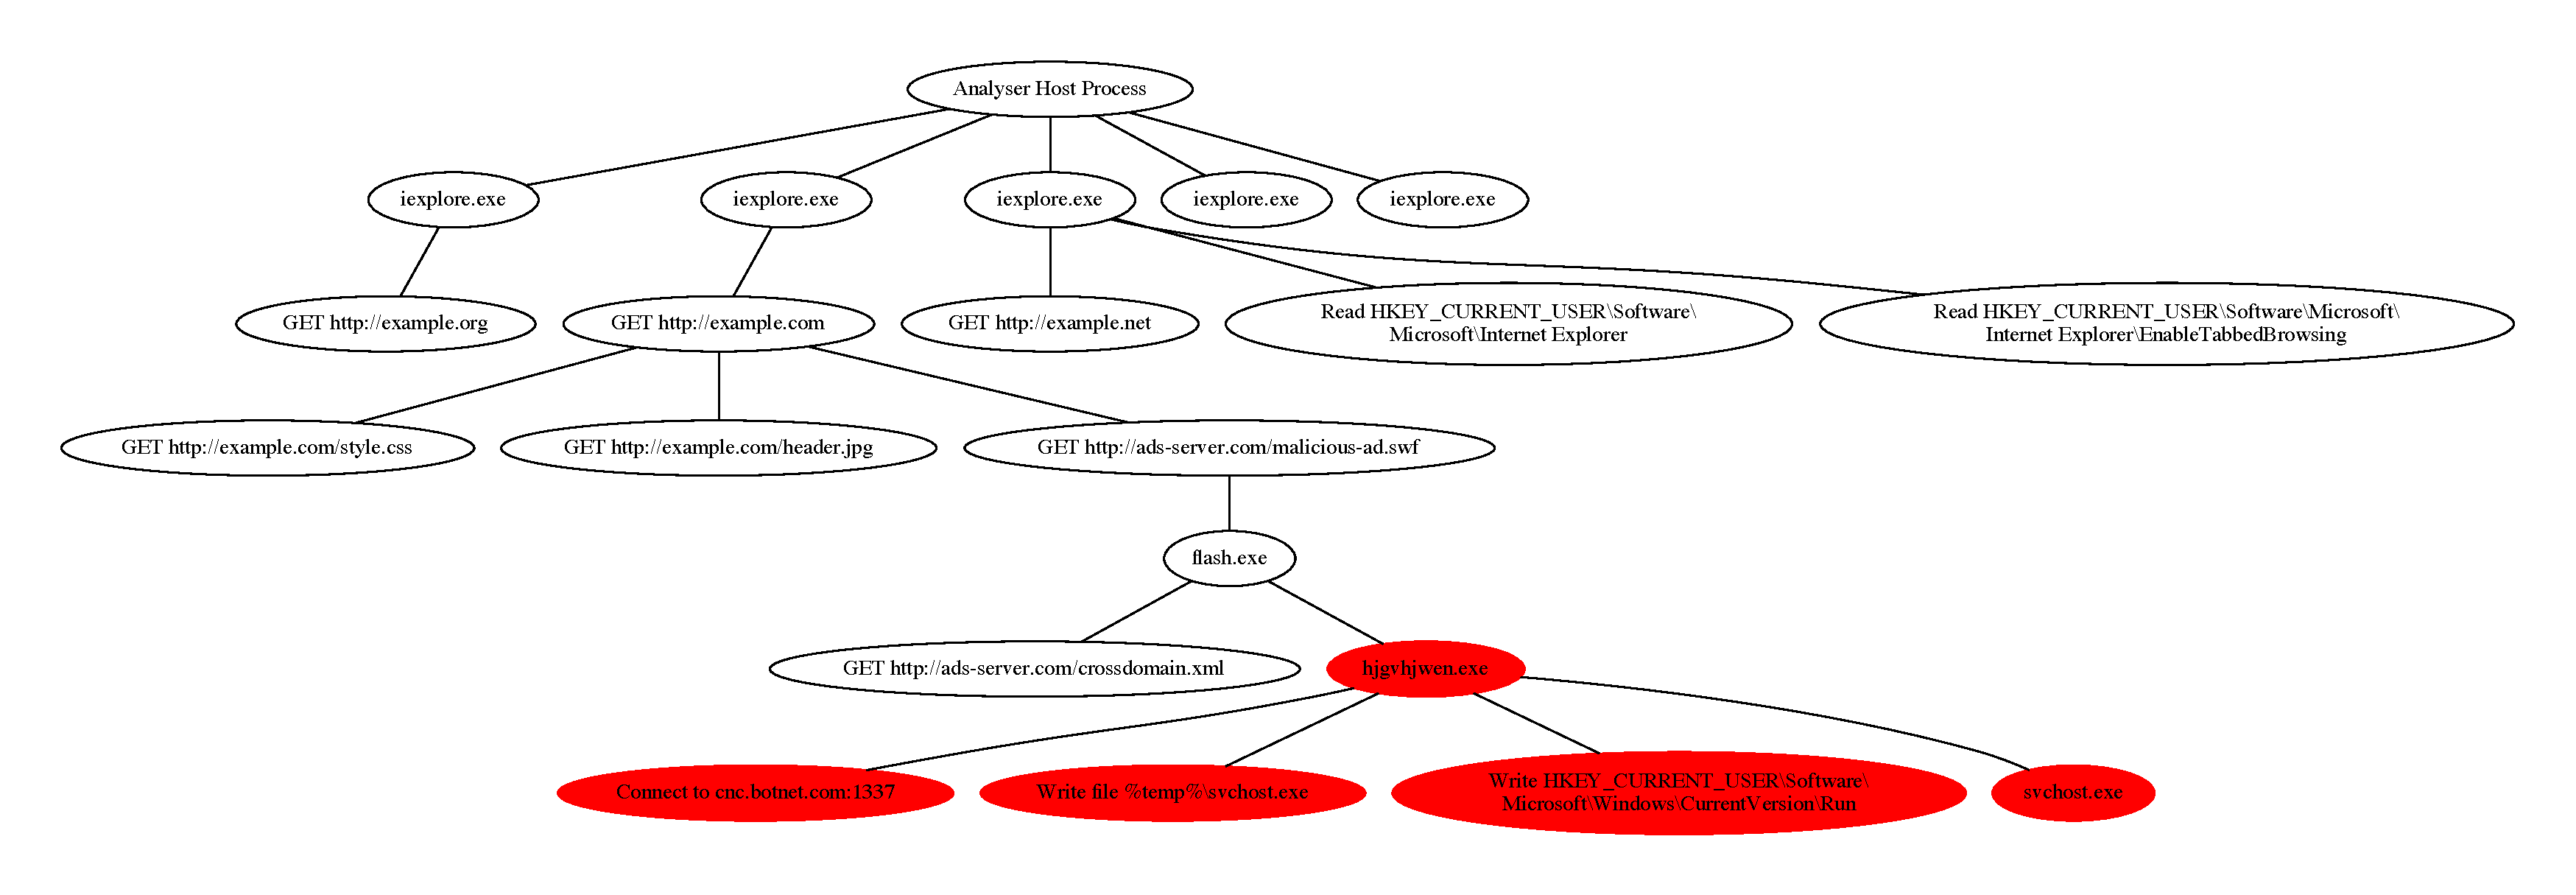
\includegraphics[width=25cm,angle=90]{Images/alg_tree}}
    \caption{An impression of how the generated graph should look. The red vertexes are marked by the imaginary analyser as malicious.}
    \label{fig:alg_tree}
\end{figure}

\stepcounter{savepage}
\pagebreak

\restoregeometry
\pagenumbering{arabic}
\setcounter{page}{\thesavepage}
